%% AMS-LaTeX Created with the Wolfram Language : www.wolfram.com

\documentclass{report}
\usepackage{amsmath, amssymb, graphics, setspace}

\newcommand{\mathsym}[1]{{}}
\newcommand{\unicode}[1]{{}}

\begin{document}

\title{Nyquist-Shannon Sampling Theorem}
\author{}
\date{}
\maketitle

\begin{abstract}The Nyquist-Shannon Sampling theorem is a fundamental one providing the condition on the sampling frequency of a band-width limited
continuous-time signal in order to be able to reconstruct it perfectly from its discrete-time (sampled) version. It stated that the sampling frequency
must be at least two times the highest frequency of the continuous-time signal spectrum.\end{abstract}

\section*{What is a Signal?}

A signal is a time/space varying function which includes some useful information. Most of signals are continuous-time ones and hence can not be either
stored (or transmitted) over realistic limited data storage (or band-limited propagation space) due to infinity of points to be processed.\\
Such signals could be of different sources or types, such as audio ones, or any real life physical measure or parameter retrieved by sensors (temp,
humidity, speed, ...).

Example of a continuous-time* signal - Mean Temperature during 2016 in Rabat, Morocco:

\begin{doublespace}
\noindent\(\pmb{\text{weatherData}=\text{WeatherData}[\{33.9716,6.8498\}, \text{{``}MeanTemperature{''}}, \{\{2016, 1, 1\}, \{2016, 12, 31\}, \text{{``}Day{''}}\}];}\\
\pmb{\text{DateListPlot}[\text{weatherData},\text{Joined} \text{-$>$} \text{True}]}\)
\end{doublespace}

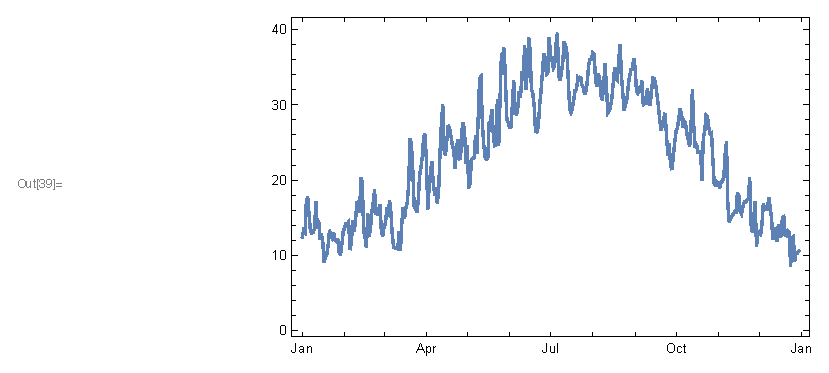
\includegraphics{TopicExploration_GhassaneAniba_gr1.eps}

In order, to process real life signals either to store or transmit, we need to a \pmb{ \textit{ sampling process}} them, making them \pmb{ \textit{
discrete-time signal}}. 

\section*{Sampling Theorem}

Sampling a continuous-time signal is getting one sample each sampling period \(T_s[s]\) , which means a sampling frequency equivalent to \(f_s=\frac{1}{T_s}[\text{Hz}]\).\\
The mean important decision to make is the sampling frequency value of \(f_s\): Indeed, if its value is too big, we{'}ll get \(f_s\) samples per
second, so large storage or large band width in order to transmit the data. If on the other hand, the value is too small, we won{'}t be able to reconstruct
the signal from the samples.\\
Hence, there is a tradeoff to make in order to minimise the needed resources (storage or frequency band-width) while being able to reproduce the
original signal from the samples.

One theorem provides an answer to this question, it{'}s the \textit{ Nyquist-Shannon Sampling Theorem} which states:

\textit{ A continuous-time signal }\textit{ \(x(t)\)}\textit{  can be sampled at a frequency }\textit{ \(f_s\)}\textit{  in order to get a discrete-time
copy of it }\textit{ \(x[n]\)}\textit{ , and afterwards be reconstructed perfectly to its original form }\textit{ \(x(t)\)}\textit{ if }\textit{
\(f_s>2f_{\max }\)}\textit{  with }\textit{ \(f_{\max }\)}\textit{  is the maximum frequency value of the }\textit{ \(x(t)\)}\textit{  signal spectrum}

Next, we{'}ll consider a \(\text{Sinc}^2\) function and see what happen to the sampled signal on the frequency domain using Fourier Transform

\section*{Sampling Process}

\subsection*{Time Domain Analysis}

Consider the function \(x(t)=\text{Sinc}^2(t)\) which represent a continuous-time signal.

Plot of the signal \(x(t)=\text{Sinc}^2(t)\):

\begin{doublespace}
\noindent\(\pmb{x[\text{t$\_$}]\text{:=}(\text{Sinc}[\text{Pi}*t]){}^{\wedge}2;}\\
\pmb{\text{Plot}[x[t],\{t,-2,2\}]}\)
\end{doublespace}

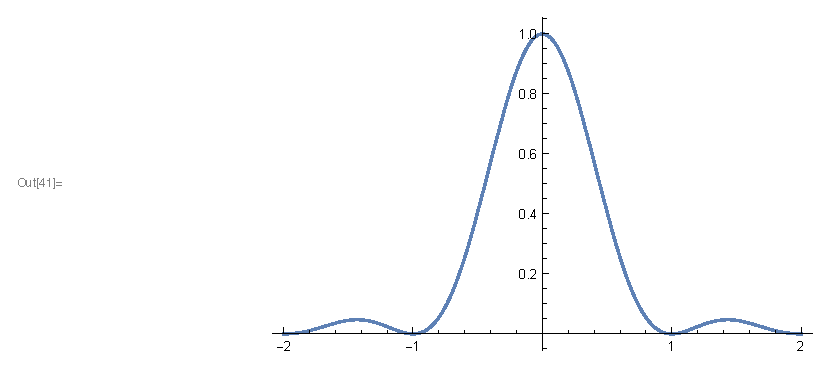
\includegraphics{TopicExploration_GhassaneAniba_gr2.eps}

Consider a sampling frequency \(f_s\)and let see what happen for different values of \(f_s.\)

Plot of the continuous-time and discrete-time (sampled) signals:

\begin{doublespace}
\noindent\(\pmb{ \text{Manipulate}[}\\
\pmb{\text{Show}[\text{DiscretePlot}[x[t],\{t, -3, 3,1/\text{fs}\},\text{PlotRange}\to \{\{-3,3\},\{-0.1,1.1\}\},\text{PerformanceGoal}\to \text{{``}Quality{''}},\text{PlotStyle}\to
\text{Directive}[\text{Orange},\text{Thick}],}\\
\pmb{\text{PlotMarkers}\to \text{Automatic}],\text{Plot}[x[t],\{t,-3,3\}]],\{\{\text{fs},15.25,\text{{``}Frequency {''}}\}, 0.5, 30,\text{Appearance}\to
\text{{``}Labeled{''}}\},\text{SaveDefinitions}\to \text{True}]}\)
\end{doublespace}

\begin{doublespace}
\noindent\(\)
\end{doublespace}

As we can see, for high values of \(f_s\) we can at least recognize visually the original continuous-time form on the \(x(t)\) signal. However, for
small values of \(f_s\) such as \(f_s=0.1\text{hz}\) for instance, we can no more visually retrieve the form of the original \(\text{Sinc}^2\) function,
with only four sample over the 20 interval duration it{'}s quite impossible to go back from samples to continuous signal. Indeed, in such case, we
are sure not satisfying the Nyquist-Shannon sampling condition.\\
In the time domain, we can somehow visually understand what{'}s happening, however, the theorem is more understandable when analyzed on the frequency
domain.

\subsection*{Frequency Domain}

The spectrum analysis of signal \(x(t)\) allows us to understand easily and even prove the theorem ourselves.

\(\text{TF}\left[\text{Sinc}^2(a t)\right] = \frac{1}{\left| a\right| }\text{tri}\left(\frac{f}{a}\right)\)

Fourier Transform of the signal \(x(t)\):

\begin{doublespace}
\noindent\(\pmb{\text{Simplify}[\text{FourierTransform}[x[t],t,\omega ]]}\)
\end{doublespace}

\begin{doublespace}
\noindent\(\frac{-2 \omega  \text{Sign}[\omega ]+(-2 \pi +\omega ) \text{Sign}[-2 \pi +\omega ]+(2 \pi +\omega ) \text{Sign}[2 \pi +\omega ]}{4 \sqrt{2}
\pi ^{3/2}}\)
\end{doublespace}

Spectrum of the signal \(x(t)\):

\begin{doublespace}
\noindent\(\pmb{\text{Plot}[\text{FourierTransform}[x[t],t,\omega ],\{\omega ,-10*2 \text{Pi},10*2\text{Pi}\},\text{PlotRange}\to \{\{-2*2\text{Pi},2*2\text{Pi}\},\{0,0.41\}\}]}\)
\end{doublespace}

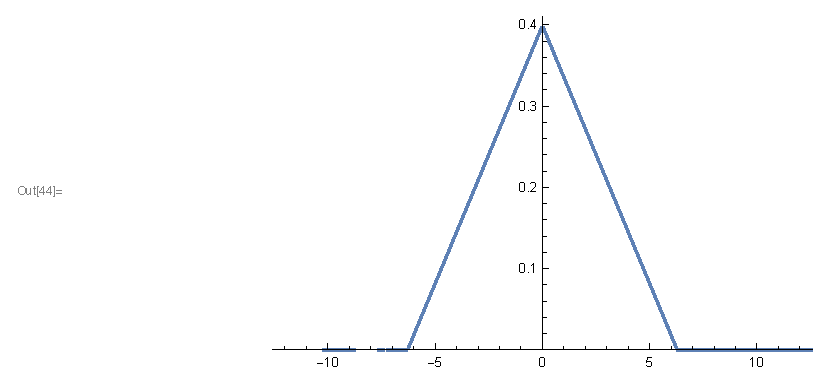
\includegraphics{TopicExploration_GhassaneAniba_gr3.eps}

Sampled signal \(x[n]\) (left) and its Fourier transform spectrum:

\begin{doublespace}
\noindent\(\pmb{\text{Manipulate}[}\\
\pmb{\text{Row}[\{\text{DiscretePlot}[x[t],\{t, -3, 3,1/\text{fs}\},\text{PlotRange}\to \{\{-3,3\},\{-0.1,1.1\}\},\text{PerformanceGoal}\to \text{{``}Quality{''}},\text{PlotStyle}\to
\text{Directive}[\text{Orange},\text{Thick}],}\\
\pmb{\text{PlotMarkers}\to \text{Automatic},\text{ImageSize}\to 340],\text{ListLinePlot}[\text{Join}\text{@@}\text{Table}[\text{Abs}[\text{Fourier}[\text{Table}[N[x[n/\text{fs}]],\{n,-4*\text{fs},4*\text{fs}+1\}]]],4],}\\
\pmb{\text{DataRange}\to \{-4\text{Pi},4\text{Pi}\},\text{PlotRange}\to \{\{-4\text{Pi},4\text{Pi}\},\{0,1.5\}\},\text{ImageSize}\to 300]\}],\{\{\text{fs},15.25,\text{{``}Frequency
{''}}\}, 0.5, 20,\text{Appearance}\to \text{{``}Labeled{''}}\}]}\)
\end{doublespace}

\begin{doublespace}
\noindent\(\)
\end{doublespace}

The spectrum of the sampled signal is a periodic form where it{'}s period is \(2\pi\), and as long as we respect the Nyquist-Shannon condition, its
form over one period is equivalent to the spectrum of the original continuous-time signal \(x(t)\). \\
Indeed, while the sampling frequency \(f_s\)is large enough, there is no overlapping between the periods of the spectrum, and then, the original
signal can be retrieved by mean of a low passband filter. However, if the sampling frequency is too low, such as \(f_s=<\)1.4 in the above example,
there will be overlapping of the spectrum, which we call an \pmb{ \textit{ aliasing effect}}. In such a case, we can no more retrieve the original
signal using a simple low-passband filter, and we need then a more powerful signal processing by means of equalization. The condition to avoid the
overlapping is that \(f_s>2f_{\max }\), which represents perfectly the Nyquist-Shannon sampling theorem.

\textit{ * The signal looks continuous on the plot but any signal processed (transmitted, stored or displayed) is always a sampled version of the
original continuous time parameter}

\section*{Reconstruction Process}

The reconstruction process consists in the generation of the original continuous-time signal \(x(t)\) from the sampled version \(x[n]\). As long
as there is no aliasing effect, a simple low passband filter is enough to retrieve the original signal

Filtering the Spectrum of the sampled signal \(x[n]\):

\begin{doublespace}
\noindent\(\pmb{\text{Manipulate}[\text{Show}[\text{ListLinePlot}[\text{Join}\text{@@}\text{Table}[\text{Abs}[\text{Fourier}[\text{Table}[N[x[n/\text{fs}]],\{n,-4*\text{fs},4*\text{fs}\}]]],2],\text{DataRange}\to
\{-2\text{Pi},2\text{Pi}\},}\\
\pmb{\text{PlotRange}\to \{\{-2\text{Pi},2\text{Pi}\},\{0,1.5\}\},\text{ImageSize}\to 300],}\\
\pmb{\text{Plot}[\text{HeavisidePi}[x/(2*\text{Pi})],\{x,-2\text{Pi},2\text{Pi}\},\text{Exclusions}\to \text{None},\text{PlotStyle}\to \text{Directive}[\text{Orange},\text{Thick},\text{Dashed}]
]],}\\
\pmb{\{\{\text{fs},8,\text{{``}Frequency {''}}\}, 0.5, 20,\text{Appearance}\to \text{{``}Labeled{''}}\}]}\)
\end{doublespace}

\begin{doublespace}
\noindent\(\)
\end{doublespace}

Depending on the existence of aliasing or not, the retrieved continuous-time signal could the perfect copy of the original or a distorted one.

Spectrum of the sample signal and the reconstructed version of the signal \(x[n]\):

\begin{doublespace}
\noindent\(\pmb{\text{Manipulate}[}\\
\pmb{\text{Row}[}\\
\pmb{\{\text{Show}[\text{ListLinePlot}[\text{Join}\text{@@}\text{Table}[\text{Abs}[\text{Fourier}[\text{Table}[N[x[n/\text{fs}]],\{n,-4\text{fs},4\text{fs}\}]]],2],\text{PerformanceGoal}\to
\text{{``}Quality{''}},\text{DataRange}\to \{-2\text{Pi},2\text{Pi}\},}\\
\pmb{\text{PlotRange}\to \{\{-2\text{Pi},2\text{Pi}\},\{0,1.5\}\},\text{ImageSize}\to 300],}\\
\pmb{\text{Plot}[\text{HeavisidePi}[x/(2*\text{Pi})],\{x,-2\text{Pi},2\text{Pi}\},\text{Exclusions}\to \text{None},\text{PlotStyle}\to \text{Directive}[\text{Orange},\text{Thick},\text{Dashed}]
]],}\\
\pmb{\text{ListLinePlot}[\text{Re}[\text{InverseFourier}[\text{Fourier}[\text{Table}[N[x[n/\text{fs}]],\{n,-4\text{fs},4\text{fs}\}]]]],\text{DataRange}\to
\{-3,3\},\text{PlotRange}\to \{\{-3,3\},\{0,1.1\}\},}\\
\pmb{\text{ImageSize}\to 300,\text{PerformanceGoal}\to \text{{``}Quality{''}}] \}],\{\{\text{fs},8,\text{{``}Frequency {''}}\}, 0.5, 20,\text{Appearance}\to
\text{{``}Labeled{''}}\}]}\)
\end{doublespace}

\begin{doublespace}
\noindent\(\)
\end{doublespace}

As long as the sampling frequency verifies the Nyquist-Shannon condition, we can reconstruct the original signal without distortion.

Further Explorations

Digital Signal Processing

Analog and Digital Modulation Techniques

Authorship information

Ghassane Aniba

23 June 2017

ghassane@emi.ac.ma

\end{document}
